%%%% -*- mode: Latex; TeX-master: "nrt14.tex"; -*-
\documentclass[11pt]{article}

\vspace{10pt}

\usepackage{fullpage,times,subfigure,fancyhdr}
\usepackage[pdftex]{color}
\usepackage{xcolor}
\usepackage{wrapfig}
\usepackage{textcomp}
\usepackage{verbatim}
\usepackage{cite}
\usepackage{times}
\usepackage{amsfonts,amsmath,amssymb,amsthm}
\usepackage{textcomp}
\usepackage{url}
\usepackage{mdwlist}
\usepackage{subfigure}
\usepackage{wrapfig}
\usepackage{xspace}
\usepackage[pdftex]{graphicx}
\usepackage{setspace}
\usepackage{enumitem}
% \usepackage[normalem]{ulem}
\usepackage{paralist}

\definecolor{dark_blue}{rgb}{0,.15,.5}
\usepackage[linecolor=dark_blue, linewidth=1.5pt, skipabove=4pt, nobreak=true]{mdframed}

\newcommand{\db}[1]{{\color{dark_blue}{#1}}}
\newcommand{\bb}[1]{{\textbf{\db{#1}}}}
\newcommand{\may}[1]{{\color{black}{\textbf{May:} #1}}}
\newcommand{\june}[1]{{\color{black}{\textbf{June:} #1}}}
\newcommand{\july}[1]{{\color{red}{\textbf{July:} #1}}}

\newcommand{\TODO}[1]{{\color{red}{\it [TODO: #1]}}}
\newcommand{\rb}[1]{{\color{green}{\it [RB: #1]}}}
\newcommand{\jv}[1]{{\color{red}{\it [JV: #1]}}}
\newcommand{\jovo}[1]{{\color{red}{\it [JV: #1]}}}


\newcommand{\sectn}[1]{\section{#1} \rfoot{\small #1 ~~ \thepage}}
%\newcommand{\sectn*}[1]{\section*{#1} \rfoot{\small #1 ~~ \thepage}}

\renewcommand{\thepage}{\arabic{page}}
\renewcommand{\thesection}{\Roman{section}}   % set the section counter to Alpha
\renewcommand{\thesubsection}{\Roman{section}(\Alph{subsection})}   % set the subsection counter to alpha
\renewcommand{\thesubsubsection}{\Roman{section}(\Alph{subsection})\roman{subsubsection}.}   % set the subsection counter to alpha
% \renewcommand{\paragraph}{\vspace{5pt}\noindent{\bb{\bf #1}}}   % set the subsection counter to alpha


\newcommand\weblink[1]{\underline{\textcolor{dark_blue}{#1}}}

\usepackage{titlesec}
\usepackage[colorlinks=true,linkcolor=magenta]{hyperref}

\titleformat{\section}
{\color{dark_blue}\normalfont\large\bfseries}
{\color{dark_blue}\thesection}{1em}{}
\titlespacing*{\section}{0pt}{10pt}{4pt}

\titleformat{\subsection}
{\color{dark_blue}\normalfont\large\bfseries}
{\color{dark_blue}\thesubsection}{1em}{}
\titlespacing*{\subsection}{0pt}{7pt}{3pt}

\titleformat{\subsubsection}
{\color{dark_blue}\normalfont\normalsize\bfseries}
{\color{dark_blue}\thesubsubsection}{1em}{}
\titlespacing*{\subsubsection}{0pt}{8pt}{4pt}

\newcommand{\para}[1]{\vspace{5pt}\noindent{\bb{\bf  #1:}}}
\newcommand{\subsubsectionnc}[1]{\vspace{5pt}\noindent{\bb{\bf #1}}}

\pagestyle{fancy}
\lhead{}
\chead{}
\rhead{}
\lfoot{}
\cfoot{}
\rfoot{}
\renewcommand{\headrulewidth}{0pt}
\renewcommand{\footrulewidth}{0pt}

\begin{document}


% {\bf \Large  Monthly Project Report for SIMPLEX DARPA Grant:} \\
% \vspace{1em}
% \large From RAGs to Riches: Utilizing Richly Attributed Graphs to Reason from Heterogeneous Data  \\

\title{Monthly Project Report for SIMPLEX DARPA Grant: \\
From RAGs to Riches: Utilizing Richly Attributed Graphs to Reason from Heterogeneous Data}

\author{PI Joshua T.~Vogelstein$^1$, Co-I Randal Burn$^2$, Co-I Carey E.~Priebe$^3$ \\
$^1$ Dept Biomedical Engineering, $^2$ Dept Computer Science, $^3$ Dept Applied Mathematics and Statistics \\
Johns Hopkins University}

% \date{May 31, 2015}

\maketitle

% \begin{center}
% ~
% \vspace{3em}
% \vspace{2em}
% \large
% \bb{Principal Investigator:} Joshua T.~Vogelstein, Assistant  Professor,\\ Department of Biomedical Engineering, Institute for Computational Medicine \\ Johns Hopins University \\
% \vspace{1em}
% \bb{Co-Principal Investigator:} Randal Burns, Associate Professor, \\ Department of Computer Science, 
% \\ Carey E. Priebe, Professor, Department of Applied Mathematics and Statistics,  
% \\ Johns Hopkins University
% \vspace{1.5em}
% \normalsize
% \end{center}

\section*{Overview}

This monthly report lists cumulative progress on our SIMPLEX statement of work.  It is organized into Tasks (captial roman numerals), their respective subtasks (captial alphabet), and subsubtasks (black bold headings).
The most recent month's progress is highlighted in red. The appendix lists all cumulative deliverables, including manuscripts, code,  data,  and resulting derivatives.




\section{Mathematical Framework}

\subsection{RAG Embedding}

\para{Tensor Factorization}

\begin{compactitem}
\item \may{While many tensor factorization algorithms exist, all of them must solve the question of: how many factors to keep.  We formulate this question as a model selection question, and are developing model selection for tensor factorization.  In preliminary work, we have written four manuscripts detailing these methods over the last couple years: \url{http://arxiv.org/abs/1312.7559}, \url{http://arxiv.org/abs/1406.6315}, and \url{http://arxiv.org/pdf/1406.6319v3.pdf}).  In May, we have begun to further develop these methods, make the code open source, and transition to more scalable implementations.}

\item \june{We are using tensor and matrix factorization techniques for two subequent inference tasks.  First, we are computing the population average graph.  Theory, simulations, and real data experiments demonstrate that we can significantly improve the current state of the art using these methods.  Second, we have developed a community detection technique using such methods.  Here, numerical experiments demonstrate a significant inference advantage, with a minimal increase in computational cost. }
\end{compactitem}



% \para{Fast JOFC and Missing Data}

% \begin{compactitem}
% \item \may{We have developed a fast numerical algorithm for the SMACOF algorithm, which is the fundamental sub-routine for running ``Joint Optimization of Fidelity and Commensurability'', which is our prefered method for embedding graphs with missing data.  We have submitted a manuscript describing our work and demonstrating its utility \cite{fjofc}.} 
% \end{compactitem}

% \para{Benchmarking}


% \begin{figure}
% \centering
% 
\includegraphics[width=0.6\linewidth]{hsbm}%l b r t
% \caption{
% Visualization of our method applied to the Drosophila connectome. We show the
% adjacency matrix (upper left), the clustering derived via ASE, projection to the sphere and kmeans
% clustering (upper right reordered), and lastly S calculated from these clusters. Clustering
% the subgraphs based on this S suggests two repeated motifs: {1, 2, 3, 5, 6, 7} and {4, 8}.
% }
% \label{fig:hsbm}
% \end{figure}


% \subsection{FlashRAG}

% \para{FlashMatrix}
% \para{FlashAttribute}
% \para{FlashR}

% \subsection{RAG Testing}

% \para{RAG 1-sample test}
% \para{RAG 2-sample test}
% \para{RAG Independence}


\section{Computational Infrastructure}

\subsection{Data Management}
\para{Dense Spatial Multi-way Arrays}

\begin{compactitem}
\item \may{In previous work, we buit a n-way dense spatial database for petascale data (\url{http://arxiv.org/abs/1306.3543}).  However, for the data types we used previously (serial electron microscopy and array tomography), the data were anisotropic.  To visualize that data, our collaborators want to downsample only along the xy dimensions, keeping the z dimension fixed.  However, for the new datasets that we will work with for this grant, CLARITY and M$^3$RI, our collaborators desire isotropic downsampling.  Thus, we have extended our infrastructure to support multiple types of downsampling, as appropriate for different datasets, including a uniform downsampling.  We have already begun using this Web-service to support alignment of CLARITY brains to the Allen Institute for Brain Science's mouse atlas, which is 25 micron isotropic.} 

\item \june{We have refactored our code such that all projects now have multiple tokens.  This is important for both MRI and CLARITY datasets, as both of them might have many tokens per dataset, corresponding to different color channels (in CLARITY), or different modalities (in MRI).  We are testing and debugging this code, which will go live shortly.}

\end{compactitem}


% \para{Sparse Multi-way Arrays}
% \para{Sparse Cutouts}

% \subsection{Remote Access and Visualization}

% \para{2D Web Visualization}
% \para{Surface Extraction}
% \para{3D Web Visualization}
% \para{Graph Web Visualization}



% \subsection{Local Access and Visualization}

% \para{API}
% \para{Downloads}
% \para{GPU 3D Visualization}
% \para{Rmote Image Annotation}

 


\section{Datafication}

\subsection{Data Ingest}

\para{Diffusion MRI}

\begin{compactitem}
\item \may{To ingest diffusion MRI data into our spatial database and corresponding annotation database, we require to additional object types in our data model.  First, a \emph{skeleton} object type, to store tracts. Second, a \emph{region of interest} (ROI) object type, to store anatomical regions.  In May, we have implemented the skeleton object type into our RAMON framework.  We have also been working with the designers of \href{http://coins.mrn.org/index.php}{COINS} and the  \href{https://www.humanbrainproject.eu/}{Human Brain Project}, to register our data with them, to enable search across datasets.} 

\item \june{We have implemented 3 new RAMON object types: \emph{skeleton}, \emph{point}, and \emph{ROI},  to subserve three different functions.  ROI can be used for MRI and CLARITY brains, for storing ROIs, and then eventually build new atlases.  Skeletons can be used to store fiber tracks from diffusion MRI, or in electron microscopy and array tomography and CLARITY, to trace microscale processes.  Points can be used to store any kind of point, be it a synapse, a cell body, or some other point.}
\end{compactitem}



% \para{CLARITY}
% \para{Calcium Physiology}
% \para{Functional MRI}


% \subsection{Data Registration}

% \para{Human Multimodal Alignment}
% \para{Mouse Multimodal Alignment}
% \para{Multi Graph Match}



% \subsection{Quality Control}




\section{Discovery}

\subsection{RAG Construction}
\para{RAG Random Walks}



\begin{compactitem}
\item \may{We have empirical evidence as well as theoretical results adapted from Rohe, Chatterjee and Yu (2011) showing that the spectrum of the graph Laplacian is robust to noise. In practice, for dimensionality reduction and embedding purposes, we build the graph Laplacian on the near neighbor matrix of a data set rather than on a dense graph, so one would like to know if similar properties hold when instead of simply adding independent entry-wise noise to a kernel matrix, we have a noisy version of the near neighbor matrix. The core idea is to use the fact that the graph Laplacian is related to the commute times of the graph: we want to show that certain kinds of noise do not change the random walks on that graph, and hence do not greatly change the Laplacian eigenmap embedding.} 

\item \june{We are investigating the computational trade-offs associated with computing normalized versus unnormalized adjacency and Laplacian matrices.  }

\end{compactitem}

% \para{RAG Sparsification}
% \para{Benchmarking}



% \subsection{RAG Summary Statistics}
% \para{RAG Moments}
% \para{RAG Motifs}
% \para{RAG Modes}



% \subsection{RAG Predict}
% \para{Nearest Neighbots}
% \para{Network of Networks}
% \para{Tensor Factorization}
% \para{Benchmarking}



\clearpage
\appendix
\section{Summary of Deliverables}


\subsection{Pre-prints and Publications}

% \bibliographystyle{ieeetr}
% \bibliography{report}
% \normalsize
% 
% \jv{turn off `References'}

% \begin{compactenum}
% \item FlashGraph publication: 
% \url{https://www.usenix.org/system/files/conference/fast15/fast15-paper-zheng.pdf} \label{pub:fg}
% \item Motif discovery pre-print: \url{http://arxiv.org/abs/1503.02115}
% \item Bayesian non-parameteric pre-print: \url{http://arxiv.org/abs/1406.7851}
% \item Scalable graph matching pre-print: \url{http://arxiv.org/abs/1310.1297}
% \item Robust vertex clustering pre-print: \url{http://arxiv.org/abs/1311.5954}
% \end{compactenum}


% \begin{compactenum}
% \item Fast JOFC: \url{http://arxiv.org/abs/1502.03391}
% \end{compactenum}

N/A


\subsection{Codes}

N/A

% \begin{compactenum}
% \item fast JOFC \jovo{url}
% \end{compactenum}

\subsection{Data and Data Derivatives}

% \begin{compactenum}
% \item	N/A
% \end{compactenum}

N/A

\section{Other Personnel}
\begin{compactitem}
\item Eric Bridgeford, BS student in Biomedical Engineering
\item Greg Kiar, MS student in Biomedical Engineering
\item Kunal Lillaney, PhD student in Computer Science
\item Keith Levin, PhD student in Applied Mathematics and Statistics
\item{Disa Mhembere, PhD Student in Computer Science}
\item{Youngser Park, research staff in Center for Imaging Science}
\item Da Zheng, PhD student in Computer Science
\end{compactitem}

% \bibliographystyle{ieeetr}
% \bibliography{report}
% \normalsize

\appendix
\section{Milestones and Deliverables}


% \clearpage
\begin{figure}[b!]
\centering
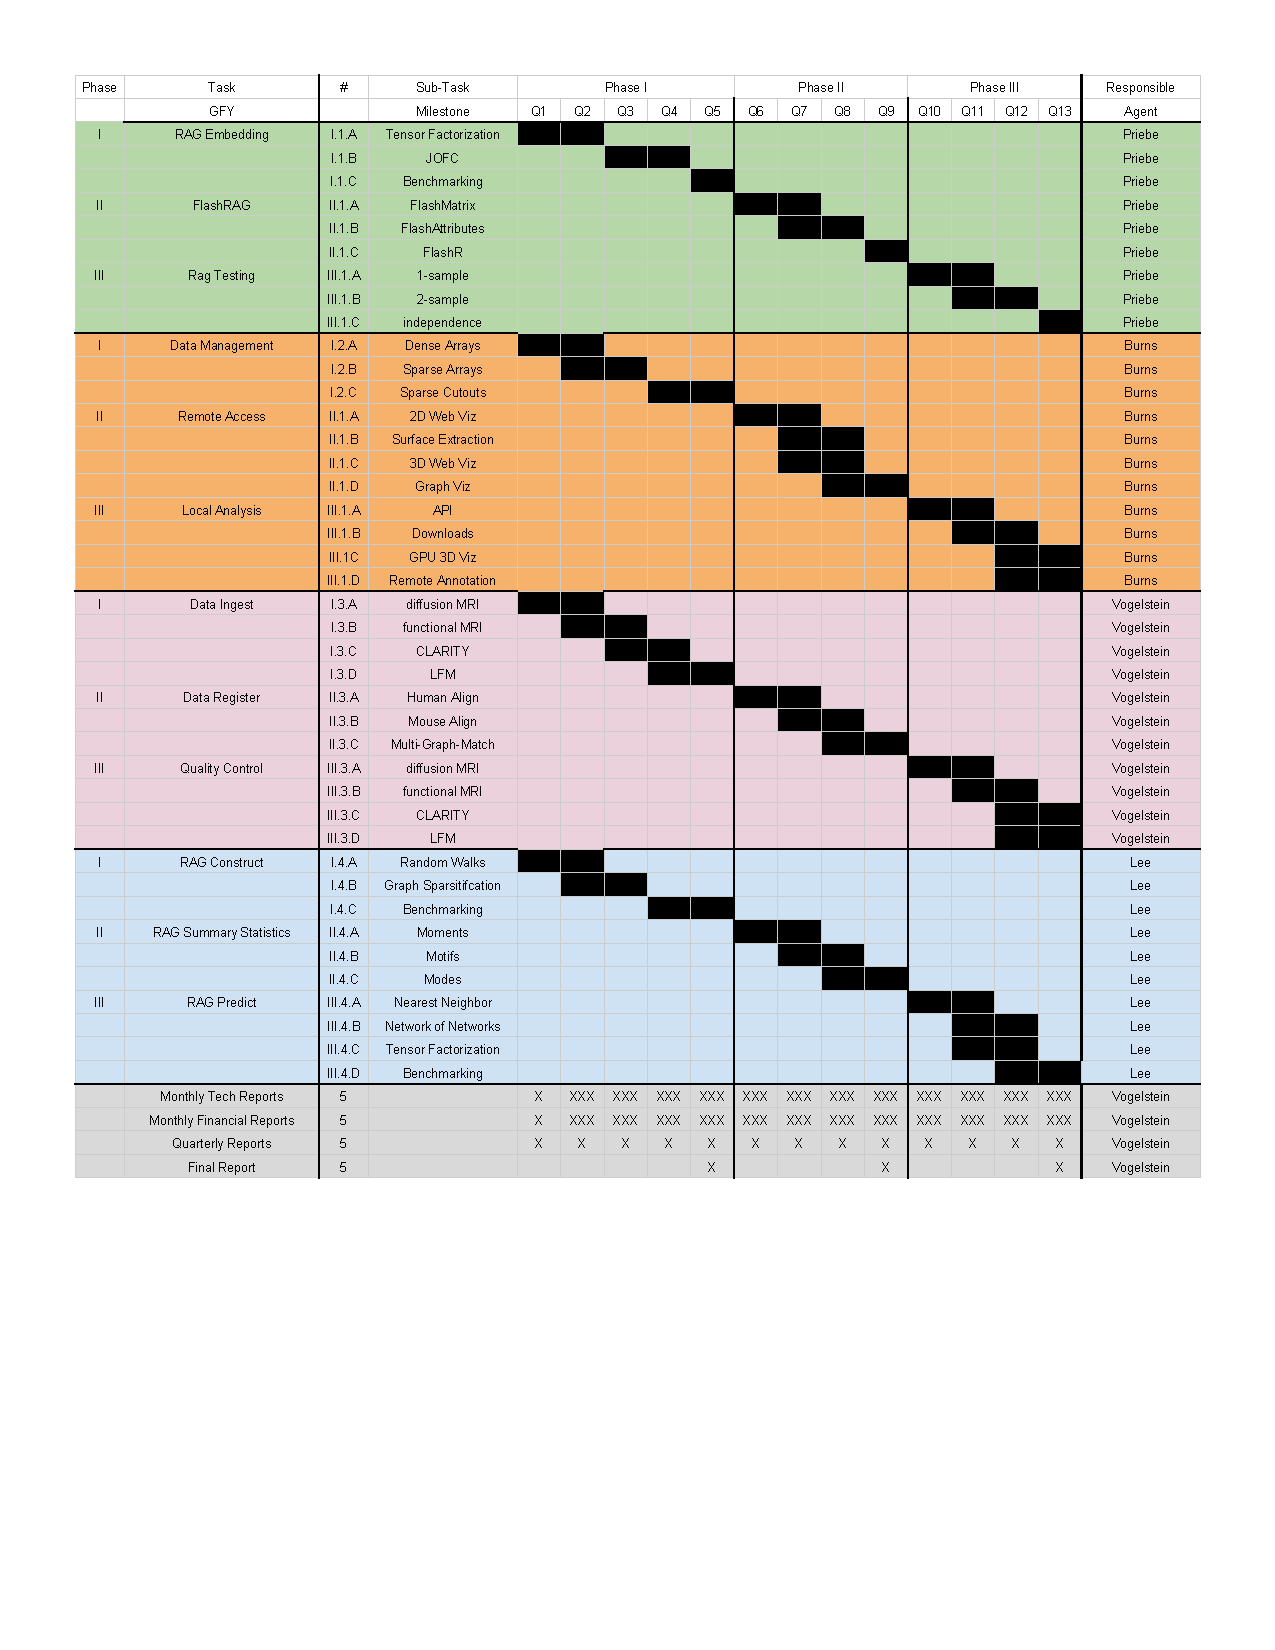
\includegraphics[width=0.6\linewidth]{SIMPLEX_Schedule}%l b r t
% \caption{.}
% \label{fig:hsbm}
\end{figure}


\end{document}
